\documentclass[10pt,conference,compsocconf]{IEEEtran}

\usepackage{graphicx}	% For figure environment
\usepackage[english]{isodate}
\usepackage[english]{babel}
\usepackage{lipsum}
\usepackage{todonotes}
\usepackage{booktabs}
\usepackage{tikz}
\usepackage{ctable}
\usepackage{subcaption}
\usepackage{amsmath}
\usepackage{float}
\usepackage[colorlinks=true, allcolors=blue]{hyperref}
\usepackage[font=scriptsize]{caption}

% Set page size and margins
\usepackage[a4paper,top=1cm,bottom=1cm,left=2cm,right=2cm,marginparwidth=2cm]{geometry}

\begin{document}
\title{\Large{Machine learning project 2:\\
Using neural networks for road segmentation of satellite images}}

\author{Luca Delabarre, Thibaud Banderet, Mateo Echeverry Hoyos}

\maketitle

\begin{abstract}
In this lab report, we propose the use of an U-Net model to segment roads in satellite images. The U-Net model is a convolutional neural network (CNN) that has been shown to be effective for image segmentation tasks. We preprocess the dataset by applying data augmentation techniques, which help to improve the performance of the model. The augmented dataset is then used to train the U-Net model. We evaluate the performance of the model using several metrics, including accuracy and F1 score. The results show that the U-Net model achieves an accuracy of 92.7\% on the test set, demonstrating its effectiveness at segmenting roads in satellite images. In addition, we also perform a detailed error analysis to understand where the model is making mistakes and identify potential areas for improvement. Overall, our results suggest that the U-Net model is a promising approach for solving this challenge.
%TODO
  %A critical part of scientific discovery is the
  %communication of research findings to peers or the general public.
  %Mastery of the process of scientific communication improves the
  %visibility and impact of research. While this guide is a necessary
  %tool for learning how to write in a manner suitable for publication
  %at a scientific venue, it is by no means sufficient, on its own, to
  %make its reader an accomplished writer. 
  %This guide should be a starting point for further development of 
  %writing skills.
\end{abstract}

\section{Introduction}
Road segmentation is the process of identifying roads in satellite images, which is an important task in many applications, such as autonomous vehicles and mapping services. By accurately segmenting roads in satellite images, we can improve the accuracy of these applications, which in turn can have a significant impact on the world.

For example, in the case of autonomous vehicles, accurate road segmentation is essential for the vehicle to be able to navigate safely. By correctly identifying roads in satellite images, the vehicle can more accurately plan its route and avoid obstacles, which can greatly improve its safety and reliability.

Additionally, accurate road segmentation can also improve the accuracy of mapping services, such as Google Maps. By correctly identifying roads in satellite images, these services can more accurately display road networks and provide more accurate directions to users. This can be especially important in areas where the road network is constantly changing, such as in developing countries.

Overall, road segmentation is an important task that has the potential to greatly impact the world by improving the accuracy of many applications. In this lab, we will explore methods for accurately segmenting roads in satellite images and evaluate their performance.
%TODO
%The aim of writing a paper is to infect the mind of your reader with
%the brilliance of your idea~\cite{jones08}. 
%The hope is that after reading your
%paper, the audience will be convinced to try out your idea. In other
%words, it is the medium to transport the idea from your head to your
%reader's head. 
%In the following
%section, we show a common structure of scientific papers and briefly
%outline some tips for writing good papers in
%Section~\ref{sec:tips-writing}.

%At that
%point, it is important that the reader is able to reproduce your
%work~\cite{schwab00,wavelab,gentleman05}. This is why it is also
%important that if the work has a computational component, the software
%associated with producing the results are also made available in a
%useful form. Several guidelines for making your user's experience with
%your software as painless as possible is given in
%Section~\ref{sec:tips-software}.

%This brief guide is by no means sufficient, on its own, to
%make its reader an accomplished writer. The reader is urged to use the
%references to further improve his or her writing skills.

%\section{The Structure of a Paper}
%\label{sec:structure-paper}

%Scientific papers usually begin with the description of the problem,
%justifying why the problem is interesting. Most importantly, it argues
%that the problem is still unsolved, or that the current solutions are
%unsatisfactory. This leads to the main gist of the paper, which is
%``the idea''. The authors then show evidence, using derivations or
%experiments, that the idea works. Since science does not occur in a
%vacuum, a proper comparison to the current state of the art is often
%part of the results. Following these ideas, papers usually have the
%following structure:
%\begin{description}
%\item[Abstract] \ \\
%  Short description of the whole paper, to help the
%  reader decide whether to read it.
%\item[Introduction] \ \\
%  Describe your problem and state your
%  contributions.
%\item[Models and Methods] \ \\
%  Describe your idea and how it was implemented to solve
%  the problem. Survey the related work, giving credit where credit is
%  due.
%\item[Results] \ \\
%  Show evidence to support your claims made in the
%  introduction.
%\item[Discussion] \ \\
%  Discuss the strengths and weaknesses of your
%  approach, based on the results. Point out the implications of your
%  novel idea on the application concerned.
%\item[Summary] \ \\
%  Summarize your contributions in light of the new
%  results.
%\end{description}


%\section{Tips for Good Writing}
%\label{sec:tips-writing}

%The ideas for good writing have come
%from~\cite{editor10,jones08,anderson04}.

%\subsection{Getting Help}
%One should try to get a draft read by as many friendly people as
%possible. And remember to treat your test readers with respect. If
%they are unable to understand something in your paper, then it is
%highly likely that your reviewers will not understand it
%either. Therefore, do not be defensive about the criticisms you get,
%but use it as an opportunity to improve the paper. Before your submit
%your friends to the pain of reading your draft, please \emph{use a
%  spell checker}.

%\subsection{Abstract}
%The abstract should really be written last, along with the title of
%the paper. The four points that should be covered~\cite{jones08}:
%\begin{enumerate}
%\item State the problem.
%\item Say why it is an interesting problem.
%\item Say what your solution achieves.
%\item Say what follows from your solution.
%\end{enumerate}

%\subsection{Figures and Tables}

%\begin{figure}[tbp]
%  \centering
%  \includegraphics[width=\columnwidth]{denoised_signal_1d}
%  \caption{Signal compression and denoising using the Fourier basis.}
%  \vspace{-3mm}
%  \label{fig:denoise-fourier}
%\end{figure}
%\begin{figure}[htbp]
%  \centering
%  \includegraphics[width=\columnwidth]{local_wdenoised_1d}
%  \vspace{-3mm}
%  \caption{Signal compression and denoising using the Daubechies wavelet basis.}
%  \label{fig:denoise-wavelet}
%\end{figure}

%%Use examples and illustrations to clarify ideas and results. For
%example, by comparing Figure~\ref{fig:denoise-fourier} and
%Figure~\ref{fig:denoise-wavelet}, we can see the two different
%situations where Fourier and wavelet basis perform well. 

%\subsection{Models and Methods}
%The models and methods
%section should describe what was
%done to answer the research question, describe how it was done,
%justify the experimental design, and
%explain how the results were analyzed.

%The model refers to the underlying mathematical model or structure which 
%you use to describe your problem, or that your solution is based on. 
%The methods on the other hand, are the algorithms used to solve the problem. 
%In some cases, the suggested method directly solves the problem, without having it 
%stated in terms of an underlying model. Generally though it is a better practice to have 
%the model figured out and stated clearly, rather than presenting a method without specifying 
%the model. In this case, the method can be more easily evaluated in the task of fitting 
%the given data to the underlying model.

%The methods part of this section, is not a step-by-step, directive,
%protocol as you might see in your lab manual, but detailed enough such
%that an interested reader can reproduce your
%work~\cite{anderson04,wavelab}.

%The methods section of a research paper provides the information by
%which a study's validity is judged.
%Therefore, it requires a clear and precise description of how an
%experiment was done, and the rationale
%for why specific experimental procedures were chosen.
%It is usually helpful to
%structure the methods section by~\cite{kallet04methods}:
%\begin{enumerate}
%\item Layout the model you used to describe the problem or the solution.
%\item Describing the algorithms used in the study, briefly including
%  details such as hyperparameter values (e.g. thresholds), and
%  preprocessing steps (e.g. normalizing the data to have mean value of
%  zero).
%\item Explaining how the materials were prepared, for example the
%  images used and their resolution.
%\item Describing the research protocol, for example which examples
%  were used for estimating the parameters (training) and which were
%  used for computing performance.
%\item Explaining how measurements were made and what
%  calculations were performed. Do not reproduce the full source code in
%  the paper, but explain the key steps.
%\end{enumerate}

%\subsection{Results}

%Organize the results section based on the sequence of table and
%figures you include. Prepare the tables and figures as soon as all
%the data are analyzed and arrange them in the sequence that best
%presents your findings in a logical way. A good strategy is to note,
%on a draft of each table or figure, the one or two key results you
%want to address in the text portion of the results.
%The information from the figures is
%summarized in Table~\ref{tab:fourier-wavelet}.

%\begin{table*}[htbp]
%  \centering
%  \begin{tabular}[c]{|l||l|l|l|}
%    \hline
%    Basis&Support&Suitable signals&Unsuitable signals\\
%    \hline
%    Fourier&global&sine like&localized\\
%    wavelet&local&localized&sine like\\
%    \hline
%  \end{tabular}
%  \caption{Characteristics of Fourier and wavelet basis.}
%  \label{tab:fourier-wavelet}
%\end{table*}

%When reporting computational or measurement results, always
%report the mean (average value) along with a measure of variability
%(standard deviation(s) or standard error of the mean).


%\section{Tips for Good Software}
%\label{sec:tips-software}

%There is a lot of literature (for example~\cite{hunt99pragmatic} and
%\cite{spolsky04software}) on how to write software. It is not the
%intention of this section to replace software engineering
%courses. However, in the interests of reproducible
%research~\cite{schwab00}, there are a few guidelines to make your
%reader happy:
%\begin{itemize}
%\item Have a \texttt{README} file that (at least) describes what your
%  software does, and which commands to run to obtain results. Also
%  mention anything special that needs to be set up, such as
%  toolboxes\footnote{For those who are
%  particularly interested, other common structures can be found at
%  \url{http://en.wikipedia.org/wiki/README} and
%  \url{http://www.gnu.org/software/womb/gnits/}.}.
%\item A list of authors and contributors can be included in a file
%  called \texttt{AUTHORS}, acknowledging any help that you may have
%  obtained. For small projects, this information is often also
%  included in the \texttt{README}.
%\item Use meaningful filenames, and not \texttt{temp1.py},
%  \texttt{temp2.py}. 
%\item Document your code. Each file should at least have a short
%  description about its reason for existence. Non obvious steps in the
%  code should be commented. Functions arguments and return values should be described.
%\item Describe how the results presented in your paper can be reproduced.
%\end{itemize}


%\subsection{\LaTeX{} Primer}
%\label{sec:latex-primer}

%\LaTeX{} is one of the most commonly used document preparation systems
%for scientific journals and conferences. It is based on the idea
%that authors should be able to focus on the content of what they are
%writing without being distracted by its visual presentation.
%The source of this file can be used as a starting point for how to use
%the different commands in \LaTeX{}. We are using an IEEE style for
%this course.

%\subsubsection{Installation}

%There are various different packages available for processing \LaTeX{}
%documents.
%On OSX use Mac\TeX{}
%(\url{http://www.tug.org/mactex/}). On Windows, use for example Mik\TeX{} (\url{http://miktex.org/}).

%\subsubsection{Compiling \LaTeX{}}
%Your directory should contain at least~4 files, in addition to image
%files. Images should be in \texttt{.png}, \texttt{.jpg} or
%\texttt{.pdf} format.
%\begin{itemize}
%\item IEEEtran.cls
%\item IEEEtran.bst
%\item groupXX-submission.tex
%\item groupXX-literature.bib
%\end{itemize}
%Note that you should replace groupXX with your chosen group name.
%Then, from the command line, type:
%\begin{verbatim}
%$ pdflatex groupXX-submission
%$ bibtex groupXX-literature
%$ pdflatex groupXX-submission
%$ pdflatex groupXX-submission
%\end{verbatim}
%This should give you a PDF document \texttt{groupXX-submission.pdf}.

%\subsubsection{Equations}

%There are three types of equations available: inline equations, for
%example $y=mx + c$, which appear in the text, unnumbered equations
%$$y=mx + c,$$
%which are presented on a line on its own, and numbered equations
%\begin{equation}
%  \label{eq:linear}
%  y = mx + c
%\end{equation}
%which you can refer to at a later point (Equation~(\ref{eq:linear})).

%\subsubsection{Tables and Figures}

%Tables and figures are ``floating'' objects, which means that the text
%can flow around it.
%Note
%that \texttt{figure*} and \texttt{table*} cause the corresponding
%figure or table to span both columns.



\section{Methods}
We use a convolutional network in order to work on this problem since our inputs are images, in fact, since our outputs are also images we use the U-Net as a general model as it is made for image segmentation \cite{wiki:u-net}.
\subsection{Preprocessing}
\label{preprocess}
Before training our model, we preprocess our data in the following way.
\subsubsection{Data augmentation}
We start by augmenting our data as we only have 100 images of 400x400 which is far from enough for a U-Net, we use the following transformations : rotations of multiples of 90 degrees, random rotations, flipping, adding gaussian or salt and pepper noise and we fill the images with black pixels so they stay rectangular. Our best working set of augmentation consists of:
\begin{itemize}
\item Rotations of 3 random angles, 90, 180 and 270 degrees
\item Flipping horizontally and vertically
\item Adding gaussian noise of two different variances (usually 50 and 200)
\item Salt and pepper with a low corruption ratio (about 2\%)
\end{itemize}
\subsubsection{Other training set}
\label{otherset}
Another way to grow our training set is by adding images from other training sets found online, namely from \cite{newtraining}. This set is far from clean (has a lot of images with white parts) and is not quite the same as the base training set we are given. We make it more usable by removing all images with white parts, but end up not using it as it is too different from our images to make our model more accurate.
\subsubsection{From images to patches}
Every image we have is 400x400 which is a big sample, it does not make much sense to give a whole image as a training item, instead we cut it into smaller patches (if the image is not a multiple of the patch size we pad it with black again). This gives us more training data without trading anything in return as long as the patches are large enough for the model to find roads easily.
\subsection{Models}
\label{models}
As explained before the U-Net is our general model but we try to train different variations of it we give each of them a name to talk about them easier later on :
\begin{itemize}
\item "Short U-Net" taken from \cite{short-unet}
\item "Multi U-Net" taken from \cite{multi-unet}
\item "Large U-Net" taken from \cite{large-unet}
\end{itemize}
The Multi U-Net model uses multiple U-Net modules to improve the performance of the model. This is achieved by concatenating the outputs of the individual U-Net modules before passing them through the final layers of the model.

The Short U-Net uses fewer layers and filters in the contracting and expansive paths. This makes the model faster to train and less prone to overfitting, at the expense of some loss of performance.

The Large U-Net model uses more layers and filters in the contracting and expansive paths. This makes the model more powerful and capable of achieving higher performance, but also makes it slower to train and more prone to overfitting.

On top of using these models as basis we also attempt to tweak them in multiple ways, for example by adding dropout layers or changing their rate, adding or removing layers or changing activation functions.
Note that we always give the preprocessed images with their values divided by 255 (since RGB values go to 255) to the model, hence each model is trained with the same exact input shape and type.

\subsection{Hyperparameters}
Here we elaborate on certain hyperparameters we tried varying and optimizing.
\subsubsection{Training set size}
As explained in \ref{preprocess}, our given training set is far too small to train our models well so we have to add more data to it. An important tradeoff to take care of is to not have too much augmented data as opposed to original data, which is why we tried using another set as explained in \ref{otherset}. We end up settling on augmenting our data from 100 to 1200 images without adding new original data, as this gave us the best results without over-fitting on the training set.
\subsubsection{Patch size}
Patch size is a very interesting hyperparameter, intuitively the best patch size would be the smallest one where it is still easy to tell a road apart from a roof of a building for example. We still try even smaller sizes such as 16x16 in order to make sure our intuition is right. The models we use also tend to work better with patch sizes as multiples of 32 so we settle on 96x96 for most of our tests.
\subsubsection{Submission threshold}
After training the model, we still need to go from our patch size to the required one (16x16) and give a single value for each of these patches, which we do by averaging the patch image and thresholding that average to either output 0 or 1. Intuitively a threshold of 0.5 sounds like the best option but because of our lack in training data, a lower threshold such as 0.2 tends to yield better results as our model does not seem so confident in his predictions (road pixels do not have values much higher than non road ones). This hyperparameter is important to maximize as it is crucial in getting a higher F1 score, the right ratio of false positive and false negative needs to be met.
\subsubsection{Others}
There are a lot more hyperparameters in our models, most of the remaining ones were optimized for training speed as they did not impact accuracy (such as learning rate, batch size, which metric to monitor while training).
\section{Results}
\subsection{Performance}
We now present different results of different variations of our model along with the best score we achieved. The main ranking statistic we use is the F1 score, which is a measure of a model's performance that takes into account both precision and recall. A high F1 score indicates that the model is able to accurately classify a large number of positive examples (i.e. roads) while also minimizing the number of false positives (i.e. non-road pixels that are classified as roads). Coincidentally the F1 score ranking gives the same ordering as ordering by accuracy on the test set (the one on AICrowd).
\begin{figure}[H]
    \centering
    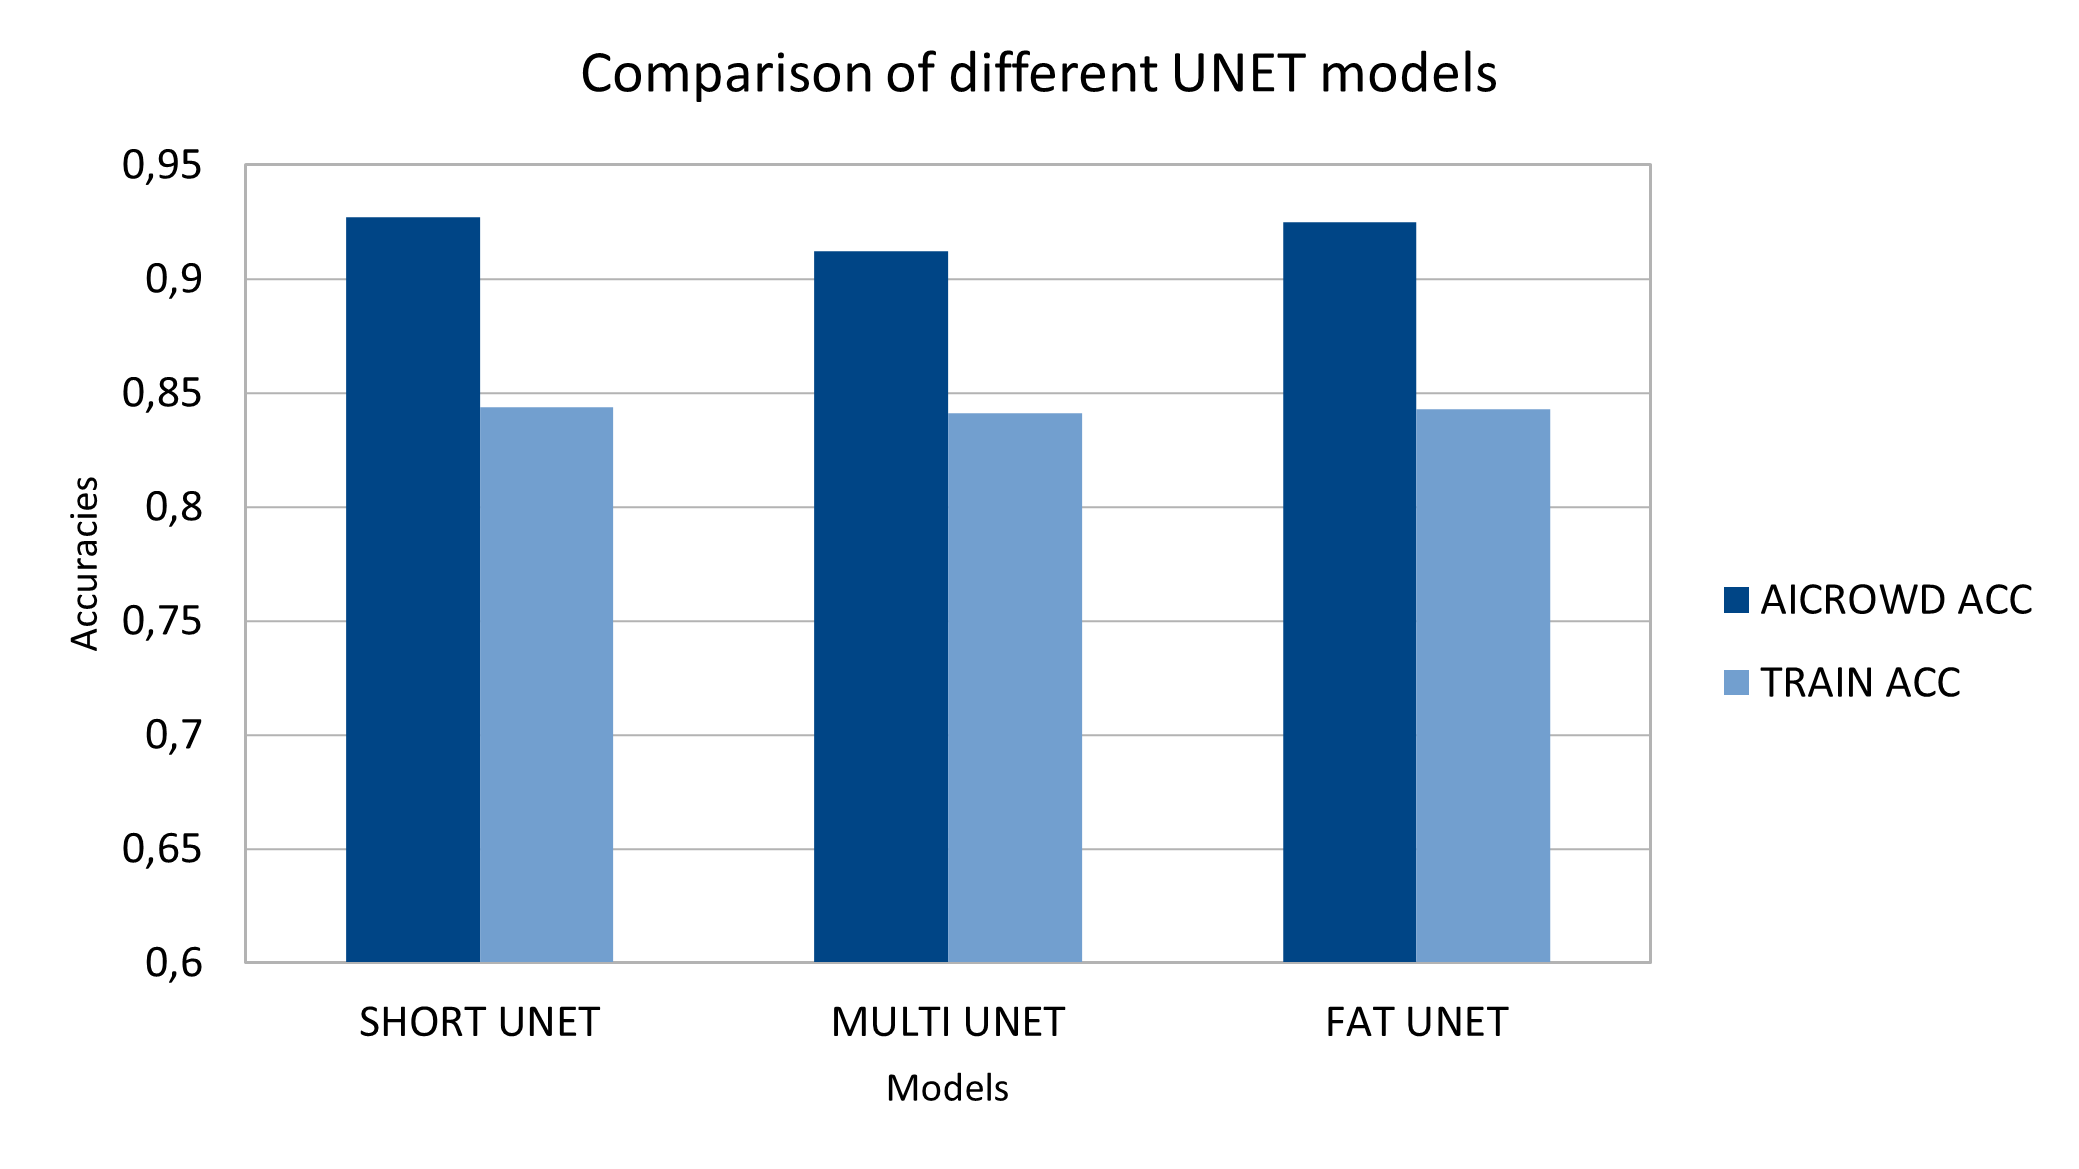
\includegraphics[scale = 0.4]{models_graph.png} %width=0.8\textwidth
    \caption{Accuracies of our various models, all using the same hyperparameters : training set augmented to 1200 images, patches of 96x96, submission threshold of 0.2, batch size of 16 and ADAM optimizer}
\end{figure}
For starters, when comparing the models we described in \ref{models}, our highest scoring model turns out to be the Short U-Net, with an F1 score of 0.859 and an accuracy of 0.927, which is the highest score we have gotten overall. The other models still have quite high scores but were mostly discarded due to the amount of time we have.
\newline
Another interesting parameter we tweaked was the submission threshold. This graph shows how much influence it has over a certain trained model.
\begin{figure}[H]
    \centering
    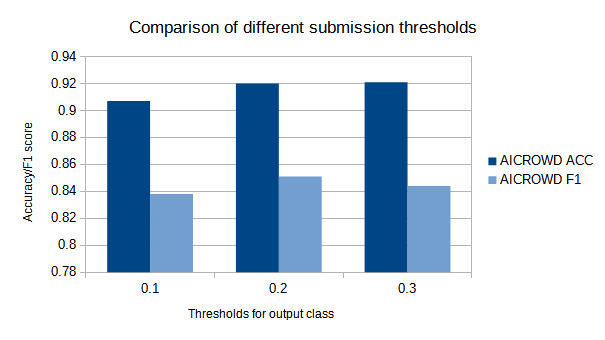
\includegraphics[scale = 0.4]{thresholds_graph.png} %width=0.8\textwidth
    \caption{Accuracy and F1 score of Short U-Net with added dropout depending on the submission threshold. The hyperparameters are : training set augmented to 1200 images, patches of 96x96, batch size of 16 and ADAM optimizer}
\end{figure}
As the graph shows, picking the right submission threshold yields drastic improvements in both F1 score and accuracy on the test set, namely a 0.2 increase from the worst to the best in the graph. This threshold was maximized on every model using a manual grid search as the only feedback we had to modify it was the AICrowd results which are limited and not linked to the training.
\newline
\label{results_data}
The last graph of results we showcase is about variations of the data augmentation for the model. There is a lot of potential variations to try here but due to the amount of submissions possible we limit ourselves to a few that we intuitively think can improve the score.
\begin{figure}[H]
    \centering
    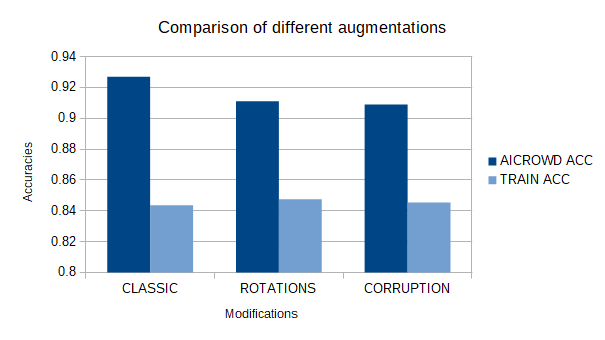
\includegraphics[scale = 0.4]{data_graph.png} %width=0.8\textwidth
    \caption{AICrowd and training accuracies of Short U-Net with different types of data augmentation : classic has 6 rotations, horizontal and vertical flips, gaussian noise with variances 50 and 200 and salt and pepper noise with rate 0.01875. Rotations removes the gaussian noise with variance 50 to replace it with another random rotation. Corruption lowers the corruptions rates to variances 10 and 50 and rate 0.01.}
\end{figure}
Here the best result turns out to be the first augmentation we tried. After looking at some predictions using this augmentation we noticed our model struggled with roads that were not vertical or horizontal, which brought the idea of adding more rotations. Another worry was about the corruption rates being too high which is why we tried lowering them too. Somehow both of these attempts resulted in worse results so we stuck with the first augmentation.
\section{Discussion}
We now discuss the results we achieved and the choices we made during this project. To begin with the models. 
\subsection{Models}
Although they were compared using the same hyperparameters, the comparison is not fully objective as each model has its own (potentially different) set of optimal hyperparameters. We however decided to mostly ignore this fact to focus on other modifications. In fact, the other high performing model turned out to be the Large U-Net which takes much longer to train and slows down our work a lot, so we decided to discard it as well.
\newline
Once the model was locked we attempted to modify it in multiple ways : 
\begin{itemize}
\item Add layers to see whether our model is large enough for the data we feed it
\item Modify the activation functions
\item Add dropout in case our model is overfitting the train data
\end{itemize}
Sadly neither of these changes led to a better score. In theory this proves that our model is large enough for our data, does not need a fancier activation function than ReLU, and that it does not overfit the training set.
\subsection{Data augmentation}
As mentioned in \ref{results_data}, there is a lot to do with data augmentation, pick how much we want to/can augment our data, pick which augmentations we want to use and how many of each along with the parameters for each augmentation. We obviously did not have the time or submissions to extensively explore all of these choices, so instead we tried slight variations in each of them.
\newline
We varied the amount of augmentation in order to get a vague understanding of whether we were augmenting too much or too little, which led to picking 11 augmentations for each image as our optimal amount. Another point to keep in mind is that trying to use a bigger model with more data takes too long to train which led to us giving up on this direction.
\newline
An intuitive way of picking augmentations is to balance them evenly and have an even amount of all of them. Which was our starting point. Once this was tested we look at predictions of the augmented data to see which augmentation is the hardest to predict and try adding more of this augmentation at the cost of removing some other ones, thus breaking the balance. As seen in the results this did not improve the scores, which suggests that keeping a good balance is more important than hyperfocusing on augmentations that are hard to train.
\newline
As for the parameters of each augmentation, most of the choices were also done out of instinct and were later confirmed to be right by comparison to others : 
\begin{itemize}
\item Random rotations were at angles between 0 and 90 as this augmentation is done to help with non vertical or horizontal roads.
\item Gaussian noise variance was brought quite high as long as the image still looked recognizable by us (200), another lower variance version was added to ease the training process.
\item Salt and pepper corruption rate follows the same idea of using a high rate that still makes the image easily recognizable to the human eye.
\end{itemize}
We then tried randomizing the rotations further by randomizing the center of rotation by a small amount. We also tried lowering the variances and corruption rates since although they look recognizable to the human eye, their values seem quite extreme for a machine learning model. However as the resulting graph in \ref{results_data} shows, these changes did not appear to be beneficial, which as said above strengthens our first instinct.
\subsection{Patch size}
The last main hyperparameter we will discuss is patch size. Yet again due to being limited we started with the following decision : the submission requires patches of 16x16 but they seem too small to be able to differentiate roads from other things. On the other hand using the full image as one data sample does not seem necessary and would result in very little training data. Therefore we lower the patch size so that roads are still easily recognizable as to maximize training data with no drawback.
\newline
Sanity checks were made to approve our method, which showed that patches of 16x16 either end with too much data to train the model within a reasonable time or much lower accuracy. Testing with full images as patches also drastically lowered the accuracy of the model. We did not have the time to grid search the optimal patch size around 96x96 however, so some further improvements might be possible in this area.
\section{Summary}

%The aim of a scientific paper is to convey the idea or discovery of
%the researcher to the minds of the readers. The associated software
%package provides the relevant details, which are often only briefly
%explained in the paper, such that the research can be reproduced.
%To write good papers, identify your key idea, make your contributions
%explicit, and use examples and illustrations to describe the problems
%and solutions.
\bibliographystyle{IEEEtran}
\bibliography{bib}
\end{document}
